\chapter{Project Planning and Design}

\section{UML Diagrams}

UML, or Unified Modeling Language, is a standardized modeling language that consists of a set of diagrams used for modeling business processes and documenting software systems, helping better communicating potential designs and architectural decisions \parencite{uml}. 

The most common UML diagrams include:
\begin{itemize}
    \item \textbf{Use Case Diagram} --- Illustrates the system's intended functionality in terms of actors, use cases, and their relationships, showing how the system delivers value to users. The diagram can also be accompanied by a use case specifications document, which provides a detailed description of each use case.
    \item \textbf{Class Diagram} --- Depicts the structure of the system by showing classes, attributes, operations, and static relationships between classes.
    \item \textbf{Sequence Diagram} --- Demonstrates how objects interact in a particular, timed sequence scenario, focusing on the messages passed between objects.
    \item \textbf{Activity Diagram} --- Represents the workflow of a target use case or business process through a series of activities, emphasizing steps, choices, iterations, and concurrency.
\end{itemize}

The student has used UML diagrams to present the stakeholders with a visual representation of the system's design and functionalities. The diagrams can be found below, under their respective sections.

\subsection{Use Case Diagram}
\begin{figure}[htbp]
    \centering
    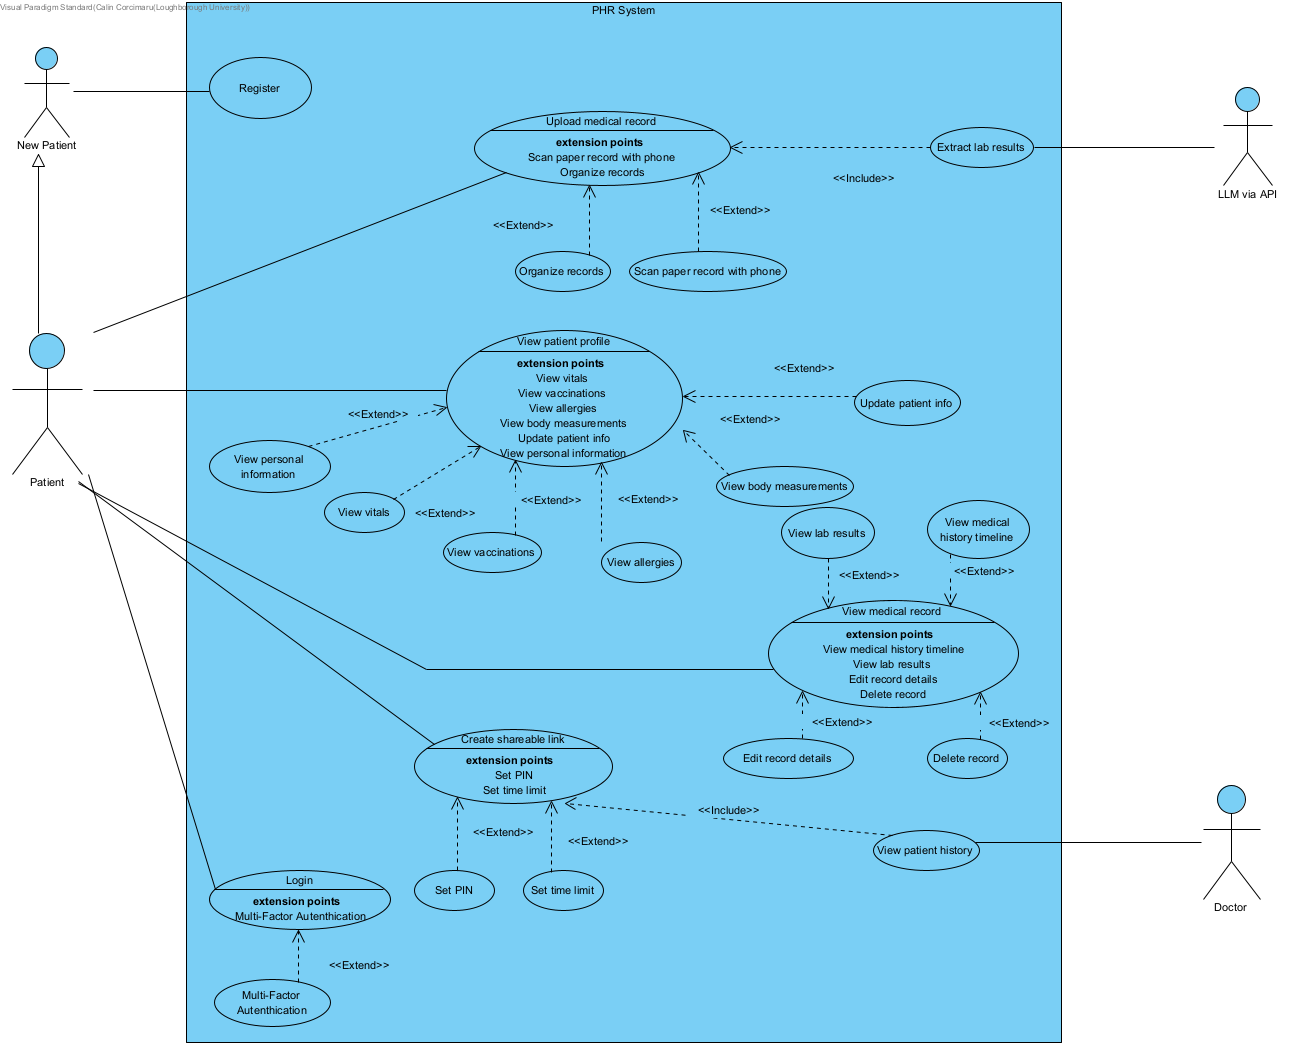
\includegraphics[width=\textwidth,height=0.7\textheight,keepaspectratio]{Use_Case.png}
    \caption{UML Use Case Diagram}\label{fig:uml_usecase}
\end{figure}

\FloatBarrier{}

\subsection{Use Case Specifications}

\subsubsection{Login}
\begin{tabular}{|p{0.2\textwidth}|p{0.7\textwidth}|}
\hline
Description & The Login use case allows the app user to log in to their existing account via their credentials, with an optional use of MFA. \\
\hline
Actors & Patient \\
\hline
Preconditions & Must have an existing account \\
\hline
Steps & 1. User enters user and password \newline
       2. User clicks on the login button \newline
       3. App validates user credentials \newline
       4. Patient enters MFA code if enabled \newline
       5. App logs user in \\
\hline
\end{tabular}

\subsubsection{Register}
\begin{tabular}{|p{0.2\textwidth}|p{0.7\textwidth}|}
\hline
Description & The Register use case allows the app user to create a new account. \\
\hline
Actors & New Patient \\
\hline
Preconditions & No existing account with the email used to register \\
\hline
Steps & 1. User enters user and password \newline
       2. User clicks on the register button \newline
       3. App validates user credentials \newline
       4. App logs user in \newline
       5. App sends verification email \newline
       6. User verifies email \\
\hline
\end{tabular}

\subsubsection{Upload Record}
\begin{tabular}{|p{0.2\textwidth}|p{0.7\textwidth}|}
\hline
Description & The Upload Record use case allows the patient to upload their medical records to the app. \\
\hline
Actors & Patient, LLM \\
\hline
Preconditions & Must be logged in \\
\hline
Steps & 1. User selects file upload (or camera scan) \newline
       2. User selects the record to upload \newline
       3. User clicks on the upload button \newline
       4. App validates the record \newline
       5. User selects the appropriate record type \newline
       6. If record type is lab result, app sends the record to LLM via API for processing into JSON format \newline
       7. App adds the record to the database \newline
       8. App shows confirmation to user \\
\hline
\end{tabular}

\subsubsection{Share Records}
\begin{tabular}{|p{0.2\textwidth}|p{0.7\textwidth}|}
\hline
Description & The Share Records use case allows the patient to share their medical records with doctors. \\
\hline
Actors & Patient, Doctor \\
\hline
Preconditions & Must be logged in and have records uploaded \\
\hline
Steps & 1. User selects option to create a share link \newline
       2. OPTIONAL\@: User selects the records to share \newline
       3. OPTIONAL\@: User adds a PIN to the share link \newline
       4. User selects time limit for the share link \newline
       5. App generates the share link \newline
       6. App sends the share link to the doctor via email \newline
       7. App shows confirmation to user \newline
       8. Doctor clicks on the share link \newline
       9. Doctor enters the PIN (if required) \newline
       10. App validates the PIN \newline
       11. App shows the records to the doctor \\
\hline
\end{tabular}

\subsubsection{View Records}
\begin{tabular}{|p{0.2\textwidth}|p{0.7\textwidth}|}
\hline
Description & The View Records use case allows the patient to view and edit their uploaded medical records. \\
\hline
Actors & Patient \\
\hline
Preconditions & Must be logged in and have records uploaded \\
\hline
Steps & 1. App provides a list of records or medical history \newline
       2. User selects record to view from list or medical history \newline
       3. App retrieves the record from the database \newline
       4. App shows the record to the user \newline
       5. OPTIONAL\@: User can view the record in a graphical format if lab result \newline
       6. OPTIONAL\@: User edits the record \newline
       7. OPTIONAL\@: User deletes the record \\
\hline
\end{tabular}

\subsubsection{View Patient Profile}
\begin{tabular}{|p{0.2\textwidth}|p{0.7\textwidth}|}
\hline
Description & The View Patient Profile use case allows the patient to view and edit their profile information, including health information such as allergies, medications, vaccinations and recorded health data like blood pressure, glucose levels, etc. \\
\hline
Actors & Patient \\
\hline
Preconditions & Must be logged in \\
\hline
Steps & 1. User selects the profile section \newline
       2. App retrieves the profile information from the database \newline
       3. App shows the profile information to the user --- vaccinations, allergies, medications, health data \newline
       4. OPTIONAL\@: User edits the profile information \newline
       5. OPTIONAL\@: User adds new health data \newline
       6. OPTIONAL\@: User deletes health data \newline
       7. OPTIONAL\@: User can view health data in a graphical format \\
\hline
\end{tabular}

\FloatBarrier{}
\clearpage

% \subsection{Class Diagram}
% \begin{figure}[htbp]
%     \centering
%     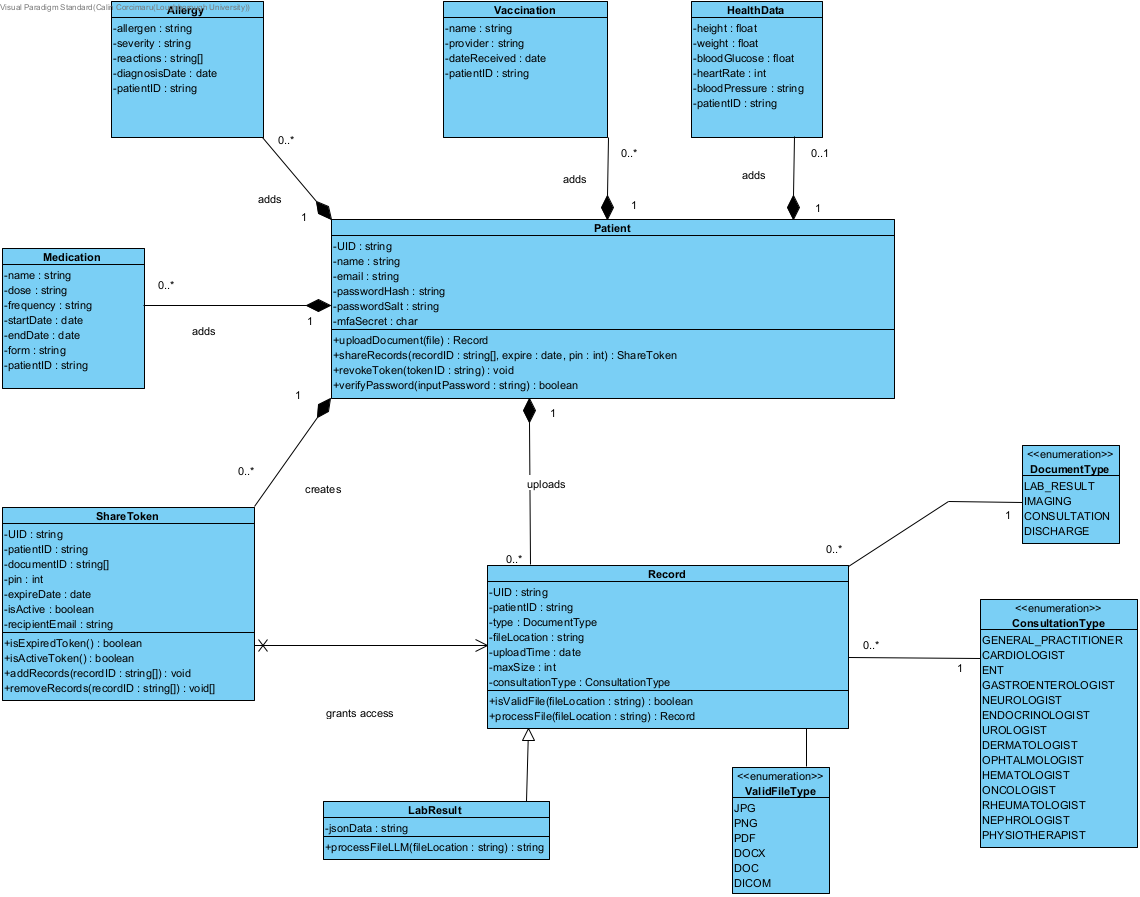
\includegraphics[width=\textwidth,height=0.8\textheight,keepaspectratio]{Class_diagram.png}
%     \caption{UML Class Diagram}\label{fig:uml_class}
% \end{figure}

% \FloatBarrier{}
% \clearpage

\subsection{Sequence Diagrams}
\begin{figure}[htbp]
    \centering
    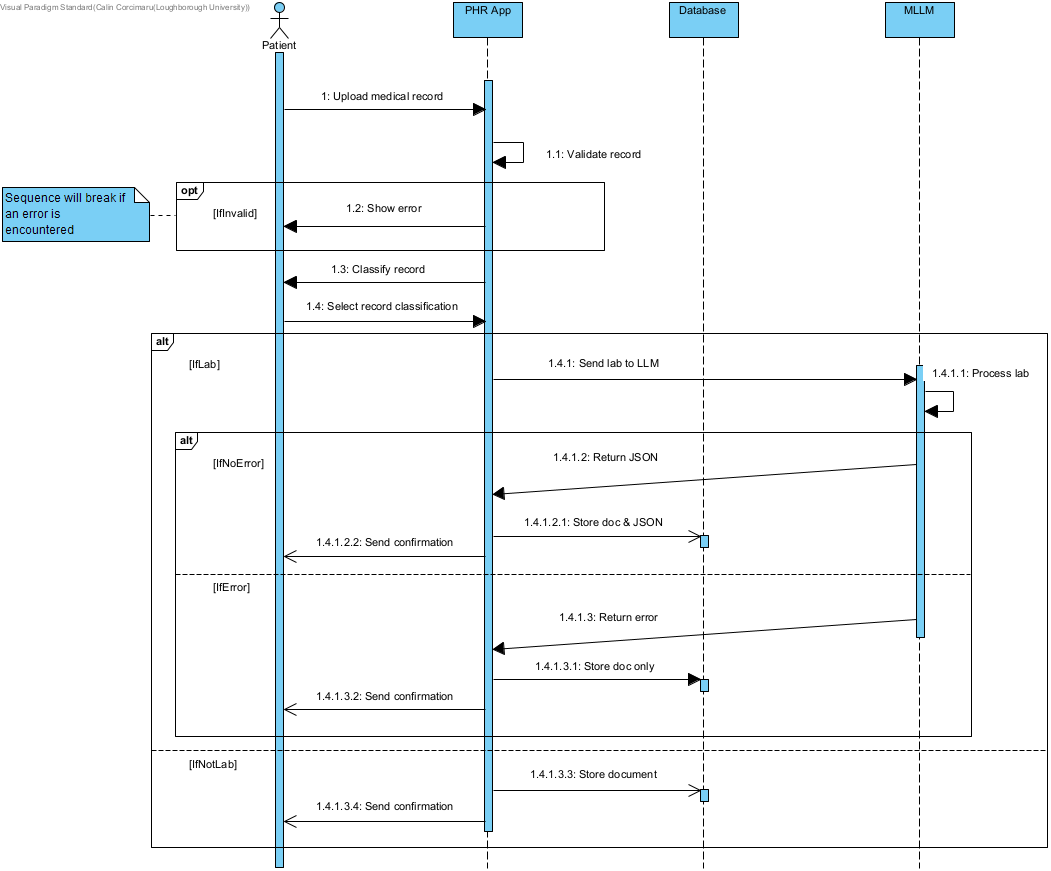
\includegraphics[width=\textwidth,height=0.8\textheight,keepaspectratio]{Sequence_upload.png}
    \caption{UML Sequence Diagram --- Upload Record Use Case}\label{fig:sequence1}
\end{figure}

\begin{figure}[htbp]
    \centering
    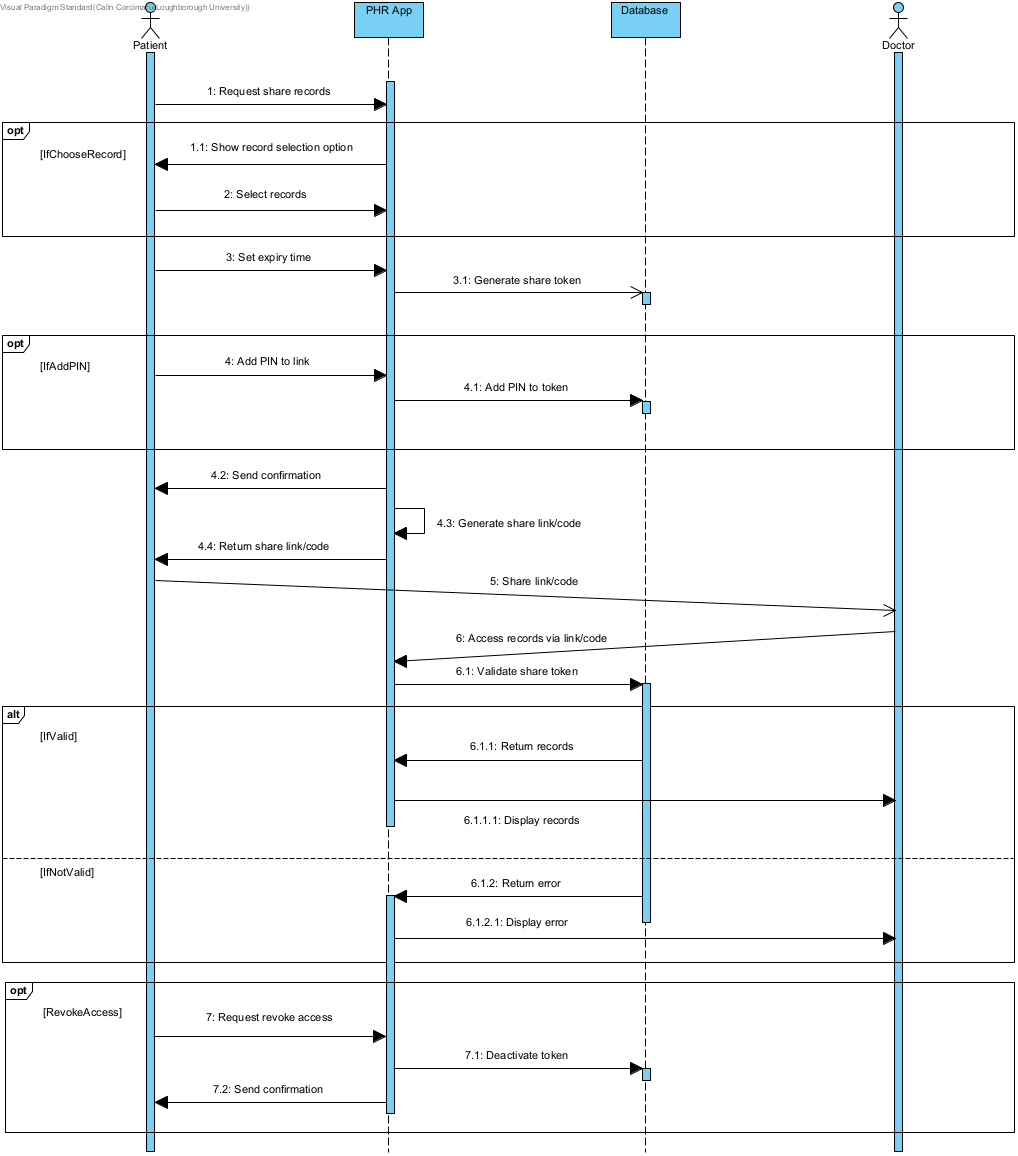
\includegraphics[width=\textwidth,height=0.8\textheight,keepaspectratio]{Sequence_share.png}
    \caption{UML Sequence Diagram --- Share Records Use Case}\label{fig:sequence2}
\end{figure}

\FloatBarrier{}

\noindent\begin{minipage}{\textwidth}
    \subsection{Activity Diagrams}
    \begin{center}
        \rotatebox[origin=c]{270}{
            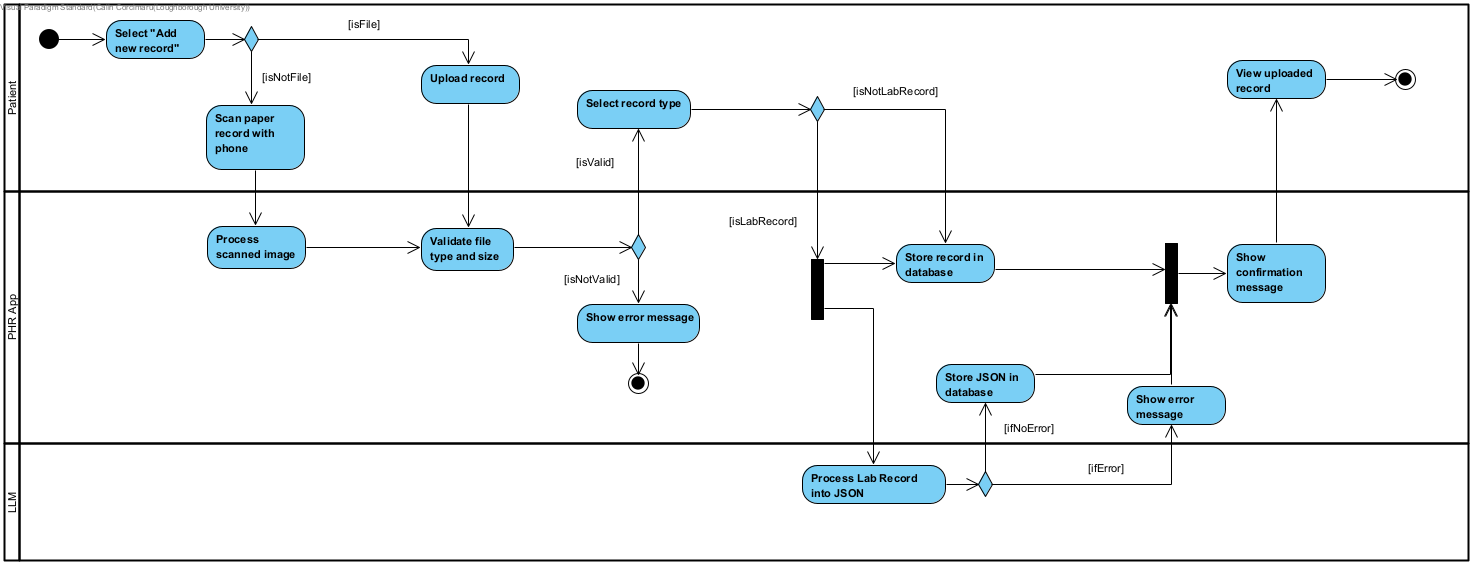
\includegraphics[width=0.9\textheight,keepaspectratio]{Activity_upload.png}
        }
        \captionof{figure}{UML Activity Diagram - Upload Record Use Case}\label{fig:activity1}
    \end{center}
\end{minipage}

\noindent\begin{minipage}{\textwidth}
    \begin{center}
        \rotatebox[origin=c]{270}{
            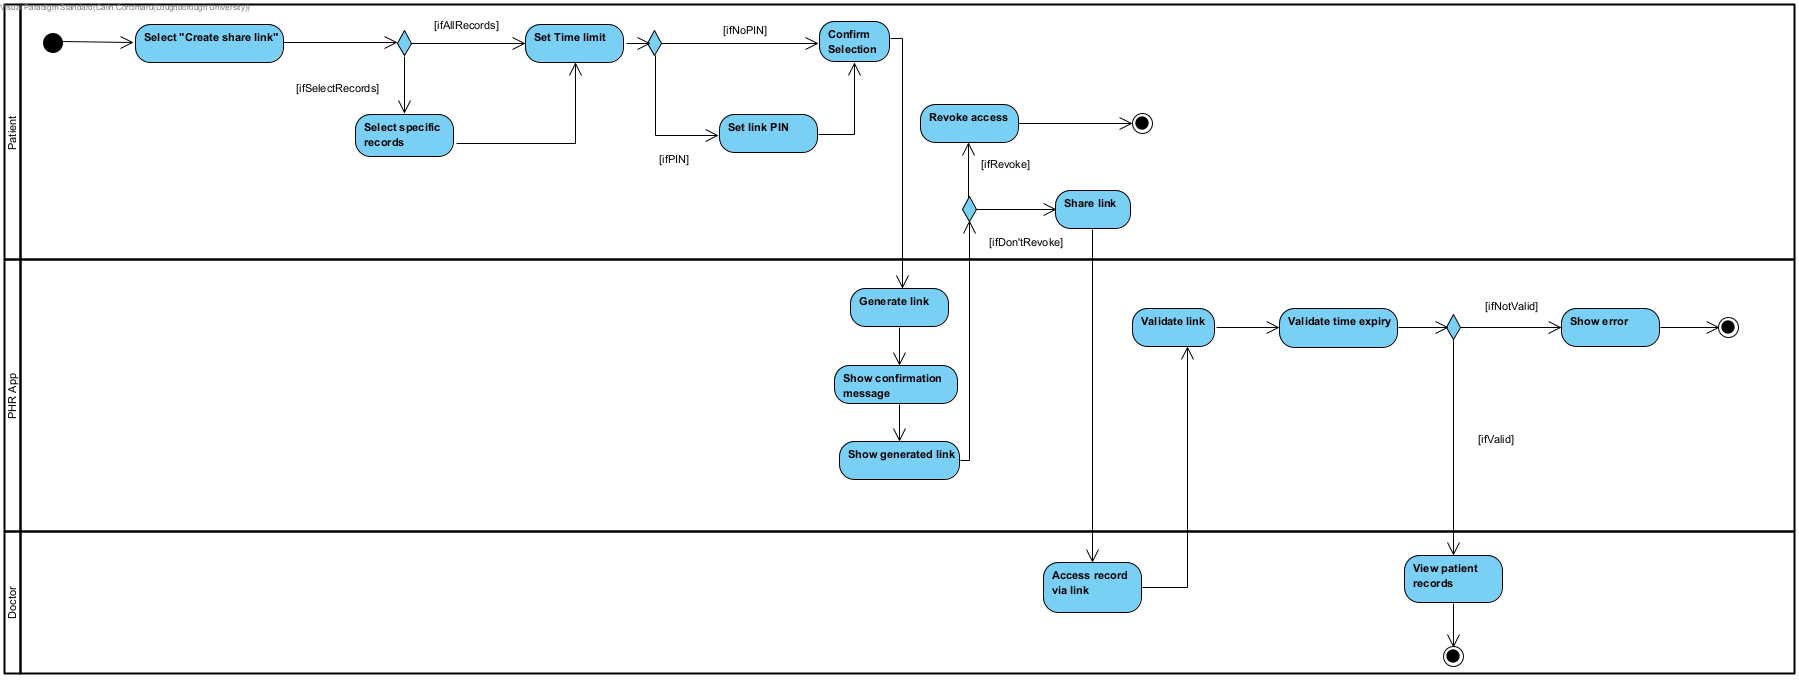
\includegraphics[width=0.9\textheight,keepaspectratio]{Activity_link.png}
        }
        \captionof{figure}{UML Activity Diagram - Share Records Use Case}\label{fig:activity2}
    \end{center}
\end{minipage}

\FloatBarrier{}

\noindent\begin{minipage}{\textwidth}
    \section{Database Design}
    \begin{center}
        \rotatebox[origin=c]{270}{
            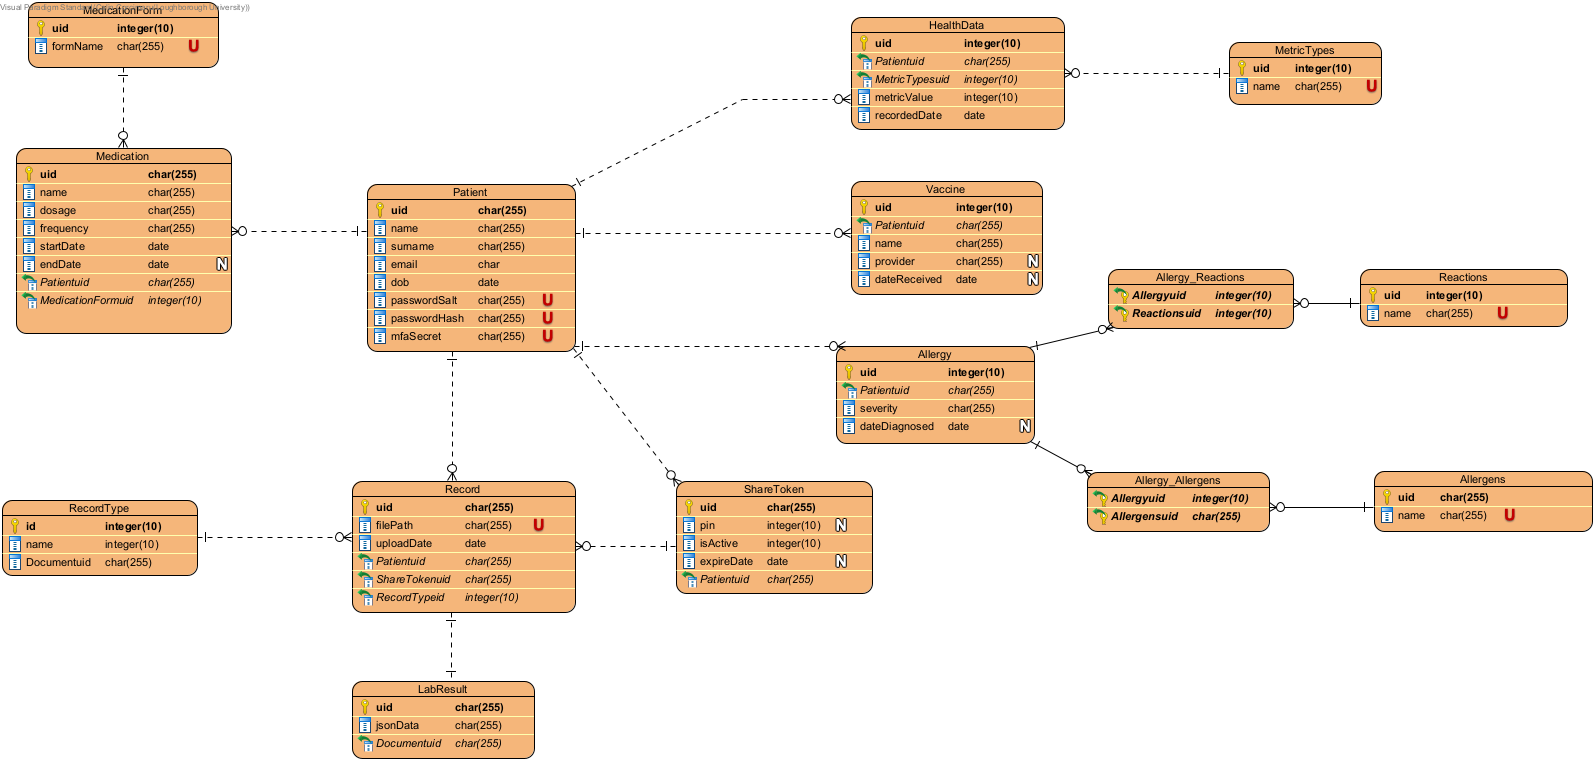
\includegraphics[width=0.9\textheight,keepaspectratio]{ERD.png}
        }
        \captionof{figure}{Entity Relationship Diagram}\label{fig:erd}
    \end{center}
\end{minipage}

\FloatBarrier{}

\section{Wireframes}

Wireframes have been used to provide a high-level overview of how the web application would look like and present some of its key functionalities. The wireframes have been created using Figma and then shown to some of the stakeholders to gather feedback. Based on the feedback received, the wireframes have been adjusted and some examples can be seen below in figures~\ref{fig:dashboard},~\ref{fig:medhistory} and~\ref{fig:lab} while the full set of wireframes can be found in the appendix~\ref{sec:wireframes}.

\begin{figure}[ht]
    \centering
    \begin{minipage}[c]{0.70\textwidth}
        \subfloat[Desktop version]{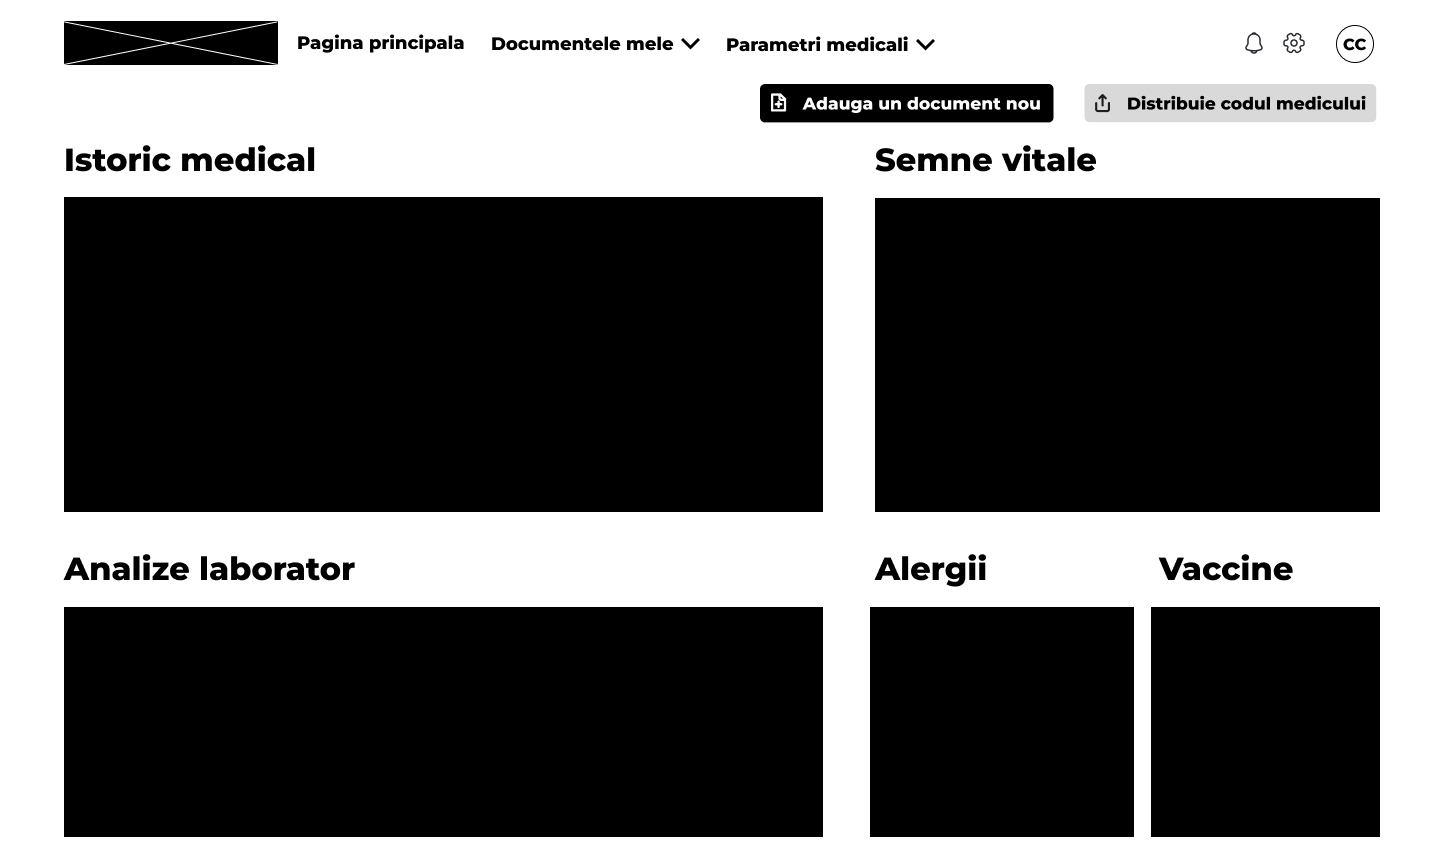
\includegraphics[width=\textwidth]{wireframes/Desktop_dashboard.png}\label{fig:dashboard-desktop}}
    \end{minipage}
    \hspace{0.05\textwidth}
    \begin{minipage}[c]{0.20\textwidth}
        \subfloat[Mobile version]{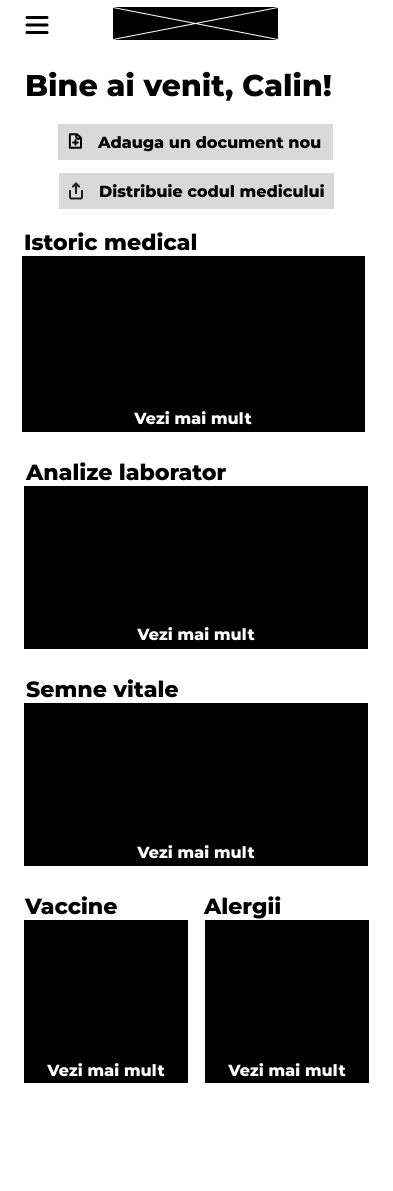
\includegraphics[width=\textwidth]{wireframes/Mobile_dashboard.png}\label{fig:dashboard-mobile}}
    \end{minipage}
    \caption{Desktop and Mobile version of the Dashboard screen}\label{fig:dashboard}
\end{figure}

\begin{figure}[ht]
    \centering
    \begin{minipage}[c]{0.70\textwidth}
        \subfloat[Desktop version]{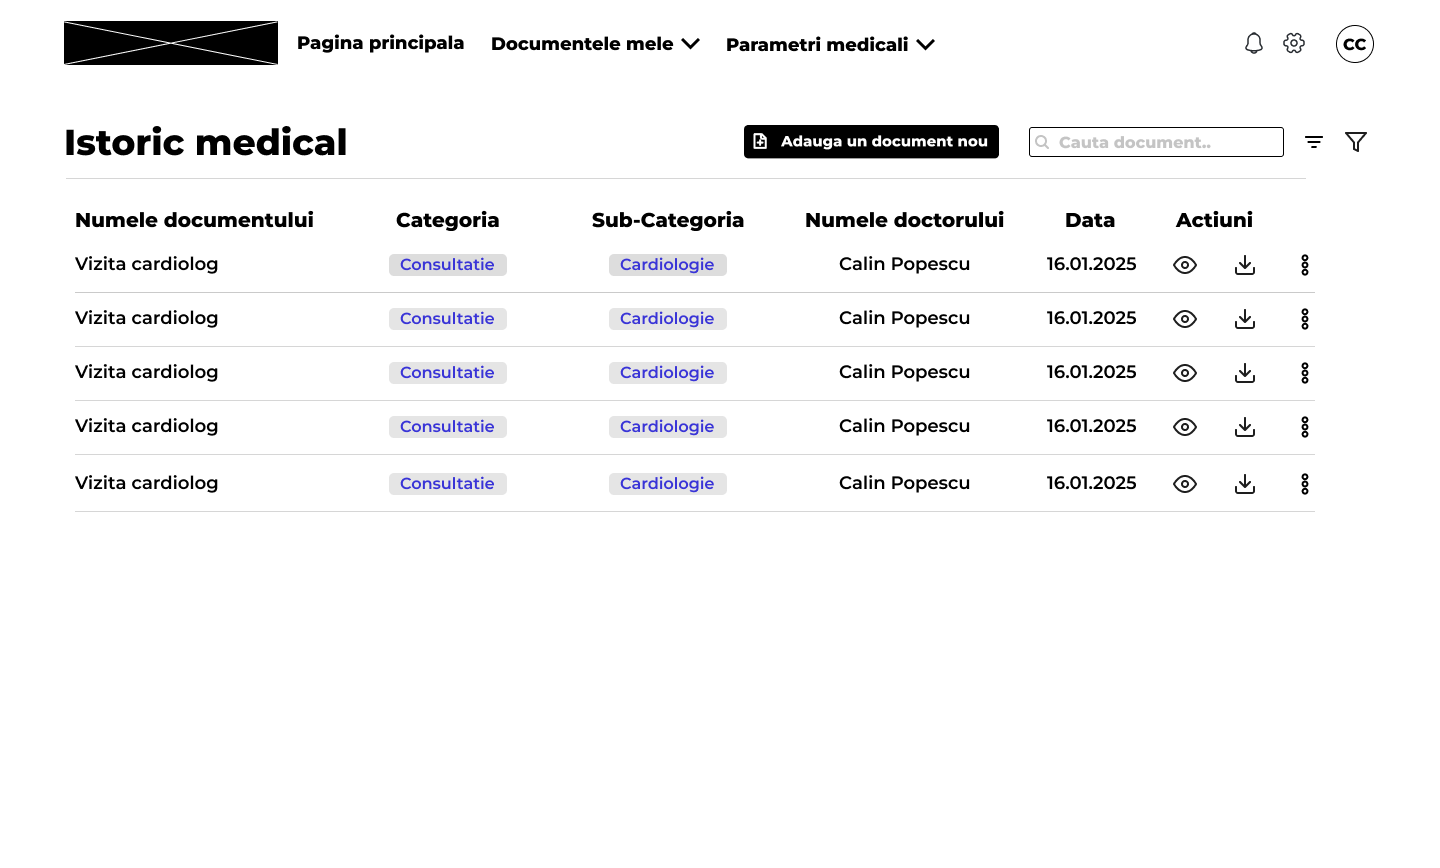
\includegraphics[width=\textwidth]{wireframes/Desktop_medHistory.png}\label{fig:medhistory-desktop}}
    \end{minipage}
    \hspace{0.05\textwidth}
    \begin{minipage}[c]{0.20\textwidth}
        \subfloat[Mobile version]{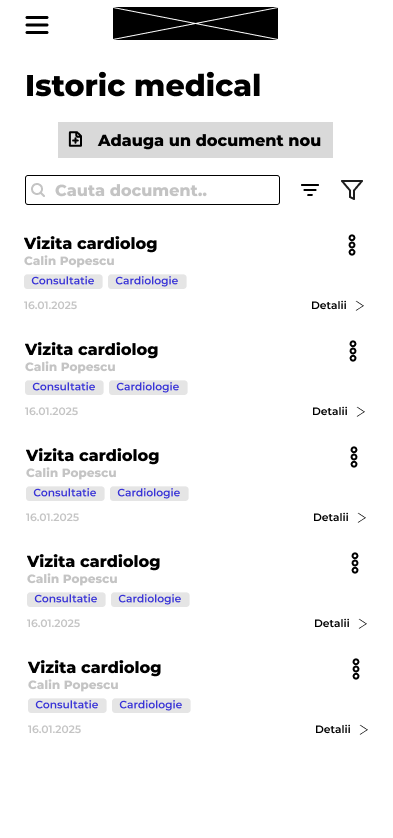
\includegraphics[width=\textwidth]{wireframes/Mobile_medHistory.png}\label{fig:medhistory-mobile}}
    \end{minipage}
    \caption{Desktop and Mobile version of the Medical History screen}\label{fig:medhistory}
\end{figure}

\begin{figure}[ht]
    \centering
    \begin{minipage}[c]{0.70\textwidth}
        \subfloat[Desktop version]{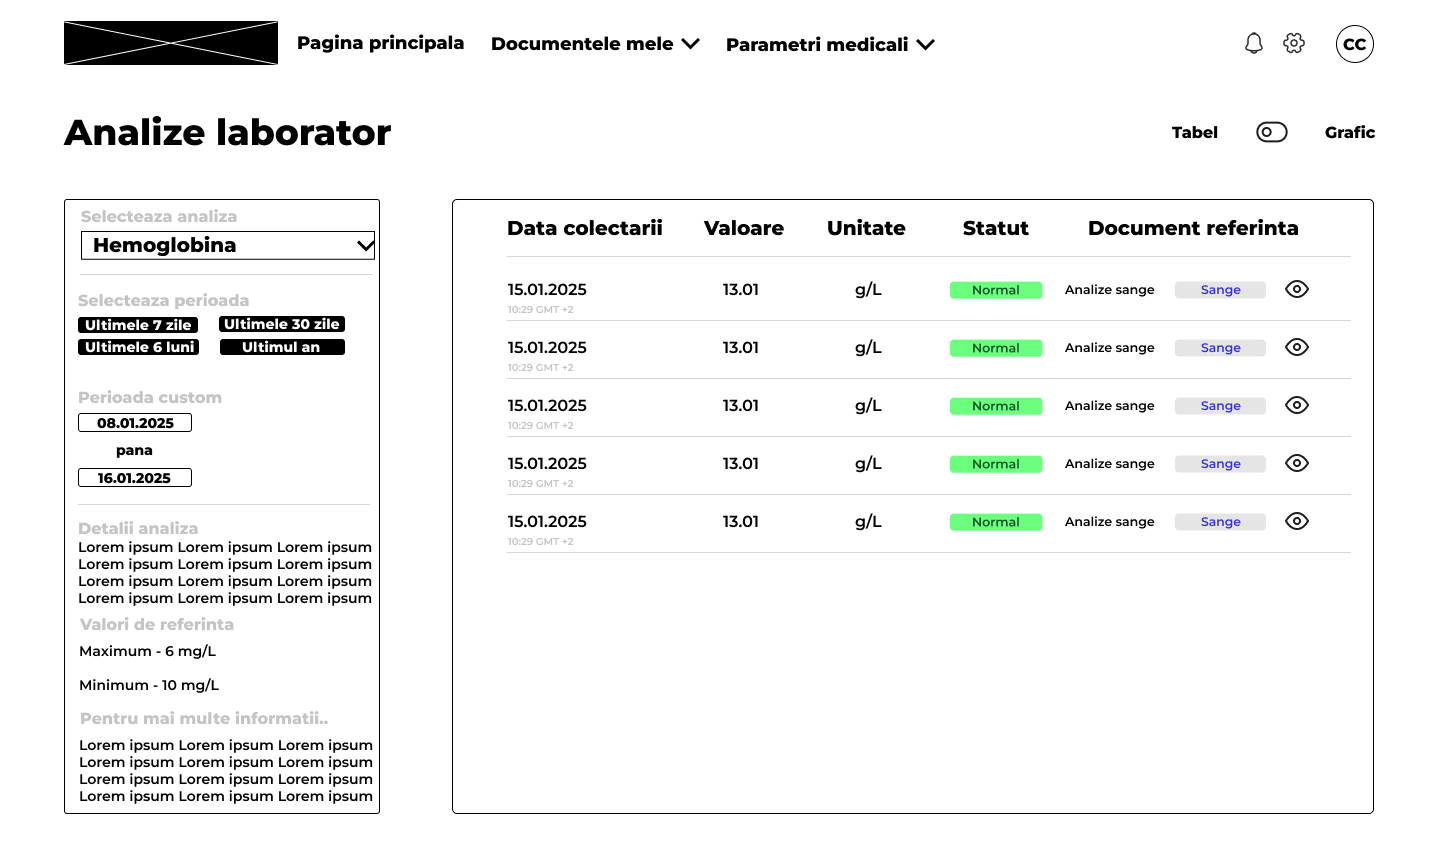
\includegraphics[width=\textwidth]{wireframes/Desktop_labTest.png}\label{fig:lab-desktop}}
    \end{minipage}
    \hspace{0.05\textwidth}
    \begin{minipage}[c]{0.20\textwidth}
        \subfloat[Mobile version]{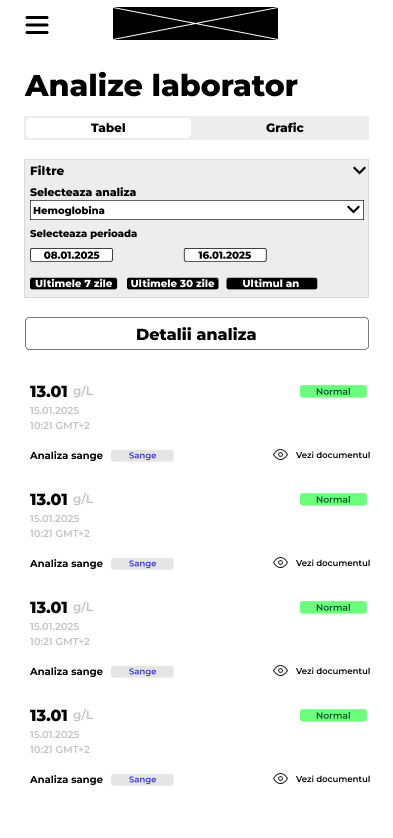
\includegraphics[width=\textwidth]{wireframes/Mobile_labTest.png}\label{fig:lab-mobile}}
    \end{minipage}
    \caption{Desktop and Mobile version of the Lab Test Results screen}\label{fig:lab}
\end{figure}

\section{Project Tech Stack}\label{sec:techstack}

Based on the research conducted in sections~\ref{sec:database},~\ref{sec:backend} and~\ref{sec:frontend}, the student has decided to use the following technologies for the project, which are shown in the diagram~\ref{fig:architecture} below.

\begin{figure}[htbp]
    \centering
    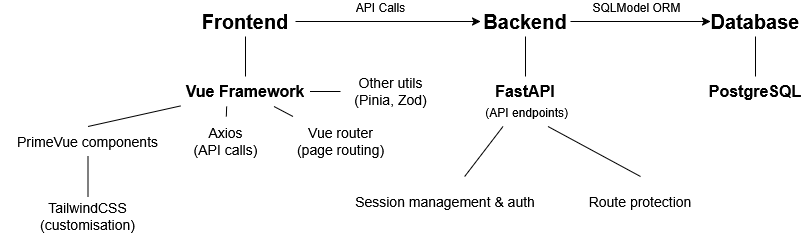
\includegraphics[width=\textwidth,height=0.8\textheight,keepaspectratio]{Sytem_architecture.png}
    \caption{Proposed System Architecture}\label{fig:architecture}
\end{figure}

In the next subsections, each part of the system will be discussed in more detail.

\subsection{Frontend}

For the frontend part of the project, the student has decided to use Vue, which is a JavaScript framework for building single-page applications (SPAs) and UIs \parencite{vue}. This framework's strengths lie in its ease of use and flexibility, with features like component and view-based architecture, element reactivity and Single File Components (SFCs) that allows HTML, CSS and JavaScript to be combined in a single \lstinline{.vue} file. Vue also boasts a large and active community, with many libaries and guides available for developers. Finally, the student has had previous experience working with Vue in their Team Project module, making it an ideal choice for this project.

Diagram~\ref{fig:frontend} below showcases how different components and libraries of the frontend will interact with each other. The next subsections will discuss each part in more detail.

\begin{figure}[htbp]
    \centering
    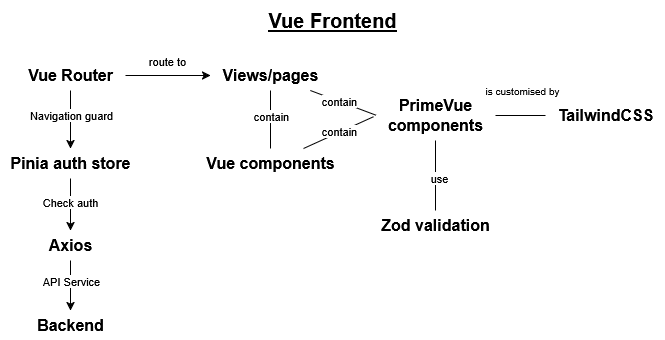
\includegraphics[width=\textwidth,height=0.8\textheight,keepaspectratio]{frontend.png}
    \caption{Interaction of Frontend Components}\label{fig:frontend}
\end{figure}

\FloatBarrier{}
\subsubsection{Vue Router}

One of the key elements of the frontend is the Vue Router. It is the official client-side router for Vue.js, which allows the user to navigate between different pages of the application without a full page reload \parencite{vuerouter}. This makes the full use of the SPA capabilities of Vue, providing a seamless and fast user experience. Similarly, Vue Router can be used to create navigation guards to protect certain routes from unauthorized access, which is crucial for the security of the application.

\subsubsection{Pinia}

The next element is Pinia, which is a store library for Vue made by the same team that created the frontend framework \parencite{pinia}. Its main functionality is to provide a way to share states across Vue components and pages. In this project, Pinia can be used to store the user's authentication status and other global states that need to be shared across the application.

\subsubsection{Axios}

The next element is Axios, which is a promise-based HTTP client for the browser and Node.js \parencite{axios}. It is used to make HTTP requests to the backend API, which is crucial for the frontend to interact with the backend. Similarly, it allows for the automatic interaction with cookies in the requests sent and responses received, which is important for the authentication process.

\subsubsection{Vue views and components}

Vue components and views (or pages) represent the foundation of the frontend for the application. Components allow to break down the UI into smaller, independent and reusable elements, which can be later combined to create the frontend of the application \parencite{vuecomponents}. Each component can be stored in a separate \lstinline{.vue} file and then imported within a view/page or another component. Views, on the other hand, represent the different pages of the application, which can be navigated to using the Vue Router.

\subsubsection{PrimeVue and TailwindCSS}

The final two elements of the frontend are PrimeVue and TailwindCSS. PrimeVue is a component library for Vue, which provides a set of pre-built components that can be used to more easily create the frontend of the application \parencite{primevue}. TailwindCSS, on the other hand, is a CSS framework that provides a set of utility classes that can be used to style the different elements of the application \parencite{tailwind}. In this application, PrimeVue provides the basic components like buttons, forms, and tables, while TailwindCSS is used to style these components.

\subsection{Backend}

For the backend part of the application, the decision was made to use FastAPI as the main framework. It is a modern and high performance web framework used in building APIs with Python \parencite{fastapi}. Based on the student's research, FastAPI seemed to be a good choice due to its ease of use, simplicity and good documentation available. The student also had previous experience with Python, making a Python-based framework an easy choice for this project. Finally, the reason for choosing a different, Python-based framework for the backend allows for more flexibility in the future, as the backend can be developed independently from the frontend and be re-used for different platforms, such as mobile or desktop applications. 

The diagram~\ref{fig:backend} below shows how different components of the backend will interact with each other.

\begin{figure}[htbp]
    \centering
    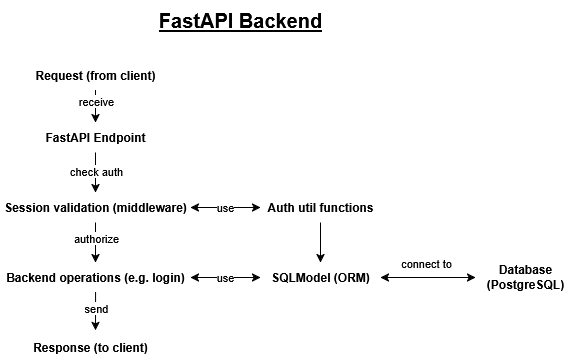
\includegraphics[width=\textwidth,height=0.8\textheight,keepaspectratio]{backend.png}
    \caption{Interaction of Backend Components}\label{fig:backend}
\end{figure}

\FloatBarrier

\subsection{Database}

For the database, the student has chosen PostgreSQL, an open source relational database system that boasts a good reputation for its reliability, wide feature set and good performance and scalability \parencite{postgres}. PostgreSQL supports a wide range of data types, including JSON and UUID, which are important for this project. Similarly, PostgreSQL offers robust security features like an access-control system, column or row-level security and secure connections with SSL, among others. 

SQLModel, a Python library built on top of SQLAlchemy and Pydantic, will be used to interact with the database. SQLModel provides a way to define database tables using classes, which are then used to interact with the database, making it easier and safer to work with databases in the backend \parencite{sqlmodel}.

\section{Project Management}

\subsection{Methodology and Tools}

Based on the research in section~\ref{sec:methodologies}, the student has decided that he will be using a hybrid approach, with Waterfall as the main methodology for planning and managing the initial part of the project, such as requirements gathering and the design of the system. The development part of the project will be done using ScrumBan, so that the student will be able to utilise elements from both frameworks. There are several reasons for this choice:

\begin{enumerate}
    \item The nature of the project --- the student is working on a project that has a limited timeframe (about 6--7 months) and is of a smaller scale. 
    \item Documentation requirements --- the student is required to document the progress during the project in this report, including the requirements gathered, design considerations and implementation decisions and outcomes. 
    \item Regulatory requirements --- the student is required to adhere to the regulations and standards of the healthcare industry, which may require extensive documentation and planning.
    \item Customer involvement --- the student will be working closely with the project stakeholder, who will be providing feedback and guidance throughout the project.
    \item Familiarity with both Agile and Waterfall --- the student has experience with both Agile (specifically Scrum and Kanban) and Waterfall methodologies, and has worked on projects that have used both approaches.
\end{enumerate}

The student will use Notion as their project management tool, which is a comprehensive workspace that allows for task management, documentation, collaboration and knowledge sharing. Notion provides a wide range of features, including templates for Agile project management, creation of Agile elements like user stories, epics, backlogs, sprints and boards, and maitaining of documentation if necessary \parencite{notion}. 

\subsection{Sprint planning}

Based on the time remaining after the completion of the literature review, requirements gathering and system design, it was decided that only 6 sprints will be able to be completed before the project deadline. The sprints will be planned as follows:

\begin{itemize}
    \item \textbf{Sprint 1} --- Will focus on choosing the tech stack, installing the necessary tools and frameworks and setting up initial project files. Additionally, a basic frontend and backend will be created, with a focus on the basic functionalities like user authentication and registration and connection with the API/database.
    \item \textbf{Sprint 2} --- Will focus on the patient profile, managing vaccines, allergies, medications and health data. The dashboard will also be created, with a basic layout and design.
    \item \textbf{Sprint 3} --- Will focus on finishing the main dashboard and the upload and viewing of medical records and medical history.
    \item \textbf{Sprint 4} --- Will focus on processing lab records with the LLM API and displaying them in tabular or graphical format.
    \item \textbf{Sprint 5} --- Will focus on sharing records with doctors through various methods like email, share links or QR codes.
    \item \textbf{Sprint 6} --- Will address any additional features or functionalities that need to be added, as well as any bugs or issues that need to be fixed.
\end{itemize}
